%======================================================================
%----------------------------------------------------------------------
%               XX                              X
%                                               X
%               XX    XXX   XXX   XXX      XXX  X  XXXX
%                X   X   X X   X X   X    X   X X X
%                X   XXXXX XXXXX XXXXX    X     X  XXX
%                X   X     X     X     XX X   X X     X
%               XXX   XXX   XXX   XXX  XX  XXX  X XXXX
%----------------------------------------------------------------------
%  	         A SKELETON FILE FOR IEEE PAPER GENERATION
%----------------------------------------------------------------------
%======================================================================

% first, uncomment the desired options:
\documentclass[%
        draft, conference,
        %submission,
        %compressed,
        %final,
        %
        %technote,
        %internal,
        %submitted,
        %inpress,
        %reprint,
        %
        %titlepage,
        notitlepage,
        %anonymous,
        narroweqnarray,
        inline,
        %twoside,
        ]{ieee}
        \usepackage{graphicx}
\graphicspath{{./Figures/}}
\centerfigcaptions

%
% some standard modes are:
%
% \documentclass[draft,narroweqnarray,inline]{ieee}
% \documentclass[submission,anonymous,narroweqnarray,inline]{ieee}
% \documentclass[final,narroweqnarray,inline]{ieee}

% Use the `endfloat' package to move figures and tables to the end
% of the paper. Useful for `submission' mode.
%\usepackage {endfloat}

% Use the `times' package to use Helvetica and Times-Roman fonts
% instead of the standard Computer Modern fonts. Useful for the 
% IEEE Computer Society transactions.
% (Note: If you have the commercial package `mathtime,' it is much
% better, but the `times' package works too).
%\usepackage {times}

% In order to use the figure-defining commands in ieeefig.sty...
\usepackage{ieeefig}

\begin{document}

%----------------------------------------------------------------------
% Title Information, Abstract and Keywords
%----------------------------------------------------------------------
\title{
      OpenComm Paper Draft}

% format author this way for journal articles.
\author[OpenComm Group]{OpenComm Group
  }

% specifiy the journal name
% \journal{IEEE Transactions on Something, 1997}

% Or, when the paper is a preprint, try this...
%\journal{IEEE Transactions on Something, 1997, TN\#9999.}

% Or, specify the conference place and date.
% \confplacedate{Ottawa, Canada, May 19--21, 1997}

% make the title
\maketitle               

% do the abstract
\begin{abstract}
Real time multi-user communication through Voice over IP grants a unique
opportunity: the ability to conduct conference calls. However, available
technologies for smart phones present challenges in their
 proprietary nature and limited features. Especially true is the ubiquitous
 problem of in-conference person identification. Although solved with video
 conferencing, current bandwidth demands make this approach highly limited with
 mobile devices.This paper presents a new application on the Android platform
 that offers a more intuitive and immersive experience. We the implementation of
 two-dimensional sound spatialization and the creation of private side chats. 
 These features will give users depth and richness of voice present in live
 conferences with hopes of providing a more natural interaction environment.
\end{abstract}

% do the keywords
\begin{keywords}
VoIP, Sound Spatialization, Android, Conferencing, Voice Communication
\end{keywords}

% start the main text ...
%----------------------------------------------------------------------
% SECTION I: Introduction
%----------------------------------------------------------------------
\section{Introduction}

\PARstart Incepted in 2005 by Cornell Professor Graeme Bailey, OpenComm is a
Human-Computer Interaction research group tackling an important question: How do
we make mobile conferencing as intuitive and immersive as possible? The short
answer is we emulate and build upon the natural conferencing experience.
Emulation of what is natural is seemingly divergent from currently established
technologies. This paper serves as a primer to OpenComm's development and
implementation of a Voice over IP(VoIP) conferencing platform featuring sound
spatialization and private side chats, all of which is currently implemented for
Android devices.

Real-time voice communication, the backbone of mobile conferencing, dates back
to the late 19th century. Despite its age, advancements in voice communication
technology have progressed slowly. On the wireless front, recent advancements in
availability have led to a surge in the number of mobile devices. Now numbering
over five billion devices across the world, cellphones�and by extension, digital
communication�are becoming an intrinsic part of our future.

That future is now. Google and Microsoft, two technology behemoths, offer users
mobile conferencing via VoIP. Free open source alternatives exist using
protocols such as the Session Initiation Protocol (SIP) . The usability of VoIP
software match�and in many cases, exceed�the traditional landline system.
However, the means of voice input and output has remained unchanged; we seem
content with faithfully reproducing the sampled voice data.

OpenComm modifies the output voice stream through the introduction of sound
spatialization. To provide for this innovative idea, OpenComm also creates a
graphical user interface that can accommodate for such changes to traditional
audio-conferencing systems.

\section{User Experience}

OpenComm provides the user with an environment that mimics and builds upon the
traditional conference room. It is not always possible for all participants in a
conference to be in one location, especially with globalization of companies and
operations. OpenComm alleviates frustrations users have with the mobile
conferencing status quo. In this section, we examine how new audio technology
and private side chats create a dynamic conference setting.

The user needs only an Android smartphone  and a set of headphones. From her
phone, the user�Alice, for example�may open up the OpenComm application to get
started. Alice can easily create a new conference by inviting people from her
contact list.

Within Alice's conference, three curved lines at the bottom of the conversation
area indicate Alice's relative position to other users, who are represented by
icons with colored borders. These icons are draggable on the screen. The
distance from Alice to each person reflects audio feedback through headphones
via a method called sound spatialization. The algorithms and implementation
comprising sound spatialization are discussed later.

Suppose Alice invites Bob, a second user, to her conference. If Alice places
Bob�s icon to her right, she will primarily hear Bob�s voice coming through her
right headphone. As she drags Bob�s icon to her left, the sound will transition
seamlessly until Bob appears to be speaking to Alice from her left. As Bob�s
icon is dragged farther away from Alice�s, his volume will decrease, and as he
is brought closer, Alice will perceive Bob to be louder. Since the sound changes
with respect to position, we deem it to be spatialized. Note that each user can
have a unique configuration of icons and is granted the power to fully
customize, as per his preferences.

In a conference scenario, Alice may want to convey some information to Bob in
private. In the real world, we are limited by the methods we can use to achieve
this. Alice may simply whisper to Bob, but only if he is sitting next to her,
Alice may also discretely send a text message to Bob as an alternative. Both of
these options are fairly obvious to their peers and are hardly foolproof. In the
virtual world, we are able to guarantee secure communication channels through
side chats.

Below the conference space is a bar containing several squares. The anchored
leftmost square always links back to the main conference. The remaining squares
are a scrollable list of the user�s side chats. Alice can create a new side chat
by clicking on the plus button and inviting members of the conference. The side
chat is similar to the main conference in functionality, including sound
spatialization. However, if Alice is in one of her side chats, only the people
in that chat can hear her. She can still hear all that is going on in main
conference at a lower volume than the voices of the people in the chat. Alice is
given free reign to say whatever she wants to Bob without the threat that
everyone else might hear her. Other users in the main conference remain unaware
of other users side chats, thus granting a further layer of anonymity to protect
any private information.

In each chat, including the main conference, the creator is initially designated
as a moderator. The moderator is the only person who has the ability to add and
remove users. Other users may send a request to the moderator to invite someone
from their contact list. If a user leaves a chat or conference for which he is
the moderator, he is given the options to either close the chat or give
moderator access to another person. With a simple, intuitive user interface,
OpenComm highlights the necessary components of real-life conferencing
experiences while enhancing privacy.

\section{Back End Changes}

Granting users the immersive experience of a real world conference is the goal
of OpenComm. As such, voice perception, the backbone of the conference, has to
be engaging. We propose a fundamentally different approach to how voice is
delivered in VoIP clients in order to meet this goal.

The current procedure in VoIP is to reproduce a digitally sampled voice without
modification. While straightforward to implement, this procedure suffers from
several drawbacks: how do we distinguish similar voices and how do we
effectively communicate in a conference environment when multiple voices are
overlayed? Furthermore, with available VoIP software such as Google Voice and
Skype, mono-channel output is simply duplicated. An easy way to verify  this is
to listen to a chat with headphones, switch the earbuds, and then listen again.
There is no difference because the left and right channels are identical.

Thus far, all varieties of VoIP implementations only reproduce the input voice
stream. We manipulate the voice stream digitally via a sound spatialization
algorithm. The output is voice localized on a two-dimensional plane for the
listener. To understand and implement the sound spatialization algorithm, we are
interested in psychoacoustics, the scientific study of sound perception.

Psychoacoustics dissects the listening experience into different areas. We are
currently not focusing on the neurological and psychological aspects, although
they make for intriguing future explorations. What we are most interested in is
the human response to sound as a mechanical wave. Human response is best
characterized by the head-related transfer function (HRTF), a complex response
function describing the ear's perception of sound. The ideal scenario for
OpenComm would be to calculate the HRTF of a user's two ears, and using that,
parameterize the spatialization algorithm accordingly. However, measuring HRTF
is currently an extremely impractical and time-consuming procedure. Our solution
is to approximate HRTF using two factors: interaural time difference and volume
difference.

There are some limitations with the spatialization algorithm. One limitation is
that the human ear's  natural localization cues are three-dimensional in nature,
taking into account azimuth, zenith, and distance. Our two-dimensional
representation is not faithful in this regard. Additionally, because sound
sources in the physical world are in 3-D, frequency responses vary according to
the shape and size of the ear. These factors are similarly unaccounted for.

The first sound spatialization factor is interaural time difference, meaning
there is a difference in when voice reaches the left and right ear, and thus, a
difference in when voice is perceived by the brain. We can emulate this natural
process with an algorithm. If we consider the angle from the right side of the
face to the center, it is positive to the right side of the nose, and negative
to the left side of the nose. For example, when the angle completely lies on a
half line from the center of the head to the left ear, it becomes -90 degrees.

\begin{figure}[h]
\centering
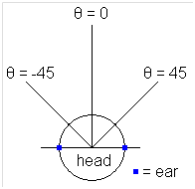
\includegraphics[width=0.4\textwidth]{1.png}

\caption{Interaural Time Delay Angles}
\end{figure}

With reference to Figure 1, the interaural time delay between two ears follow
the formula:

\begin{equation}
\textrm{interaural time delay} = \frac{\textrm{radius of head}}{\textrm{speed of
sound}} \times (\theta + sin(\theta))
\end{equation}

Negative delay means that the left ear first hears the sound. Here, $\theta$ is
in radians.

 By calculating the distance to both ears and the speed of sound, our algorithm
computes the difference in time for any source on the 2-D plane to reach the
left and right ears, giving a virtual soundstage.

Volume difference is the second factor used to approximate HRTF. Volume, or
sound pressure, is inversely proportional to the distance. In plain terms, sound
is less loud the farther away it is. The relationship between volume differences
and sound localization called the interaural level difference. Our calculation
is dependent on the distance of each ear from the sound source.

The difference in distance between two ears is calculated from the interaural
time delay. Since the speed of sound was assumed to be constant, the difference
in distance can be obtained from the time. From this, the actual distances of
each ear from sound source can be calculated.

\begin{equation}
\textrm{distance difference = interaural time delay} \times \textrm{speed of
sound}
\end{equation}
\begin{equation}\textrm{distance to left ear = d} + \frac{\textrm{distance
difference}}{2}\end{equation}
\begin{equation}
\textrm{distance to right ear = d} - \frac{\textrm{distance
difference}}{2}
\end{equation}

From here, we set the appropriate volume for each ear individually according to
our algorithm.
\section{Implementation}

Our Android application combines OpenComm's front-end and back-end changes with
an established VoIP framework. For OpenComm, the VoIP framework is a system of
Extensible Messaging and Presence Protocol (XMPP), Jingle, and Real-Time
Transport Protocol  (RPT) protocols on the Jabber server. The end result allows
conference calls to be established. Built on top of this framework are the sound
spatialization algorithm and the graphical user interface, featuring private
side chats.

The server backbone of OpenComm is Jabber. Jabber is the original name of the
current XMPP server project and is now one of the biggest nodes on the open XMPP
network. The key service Jabber provides is a secure server client supporting
the XMPP protocol, the basis of a conference chatroom.

XMPP handles session negotiations and connections management. We utilize Smack,
an open source client library for instant messaging and presence that is an
extension of XMPP. The Smack library is ported for the Android platform via the
asmack package with libraries for connection management, authentication
mechanisms, and the creation of multi-user-chat (MUC) rooms.

The Jingle protocol is an extension to XMPP that allows Jabber clients to set
up, manage and tear down VoIP sessions. This involves the sending, receiving and
parsing of Jingle packets. Sending and receiving packets is taken care of via
asmack. However, the parsing of packets presents a more challenging problem. The
existing Jingle libraries are unfeasible for OpenComm, so an original library
has been developed. This Jingle library accomplishes three major things:
construction of a Jingle packet, the parsing of packets, and the determination
of events and appropriate transitions based on  packets.

The combination of XMPP, Jabber and Jingle protocols allow for session
connection and management. OpenComm received its inspiration for sending and
receiving voice packets from Sipdroid, a free SIP/VoIP client for Android. We
utilize Sipdroid's implementation, encoding the packets using the G.711 codec at
64 Kbits/second. To transport the encoded packets, OpenComm uses RTP, which is
built on top User Datagram Protocol (UDP). UDP is a defined internet transport
protocol (IP), hence Voice over IP . However, the fact that Android does not
support multicast addressing (having multiple recipients for a single source)
complicates our implementation. This problem is solved with multiple streaming
and receiving threads.

OpenComm's two unique infrastructures, including sound spatialization and
private side chats, are implemented above this robust VoIP framework. On the
back-end, we use the Android AudioTrack class to do the heavy lifting. Two
AudioTrack objects handle the left and right sides separately. Interaural time
difference is taken into account by having a time difference between the two
streams. The existing setStereoVolume() method in AudioTrack succinctly takes
care of the volume differences.  Combining the volume and time difference allows
OpenComm to spatialize a user icon on the interface into a sound source in 2-D
space.

The front-end implementation of our application involves Human-Computer
Interaction(HCI) Design and GUI development on the Android platform. The
keystone of our HCI Design is the creation of side chats that operate and behave
congruently with the main conference chat. Alongside with the chat screens, our
application features a minimalistic theme. The GUI itself is designed using
vector graphics with an emphasis on consistency and cleanness. As previously
discussed, our front-end implementation emphasizes the user experience.

\section{Conclusion}

The potential for virtual VoIP conferencing is unlimited. Current
implementations reproduce the input without modification. OpenComm diverges from
this norm, attempting to provide a more immersive experience through spatialized
sound and an intuitive user experience.

% try out a theorem...
% \newtheorem{IAD}{Theorem}
% 
% \begin{IAD}[Interaural Time Delay Formula]
%   Consider the system ...
% \end{IAD}
% 


% do the biliography:
\bibliographystyle{IEEEbib}
\bibliography{my-bibliography-file}

% where ``my-bibliography-file.bib'' is the name of the file with all the 
% BibTeX entries.

% do the biographies...
% \begin{biography}{Gregory L. Plett}
%   A bio with no face...
% \end{biography}

% If you want a picture with your biography, then specify the name of
% the postscript file in square brackets. That is, uncomment the
% following three lines and change the name of "face.ps" to the name of 
% your file.
%\begin{biography}[face.ps]{Gregory L. Plett}
%  A bio with a face...
%\end{biography}

%----------------------------------------------------------------------
% FIGURES
%----------------------------------------------------------------------
% There are many ways to include figures in the text. We will assume
% that the figure is some sort of EPS file.
%
% The outdated packages epsfig and psfig allow you to insert figures
% like: \psfig{filename.eps} These should really be done now using the
% \includegraphics{filename.eps} command.  
%
% i.e.,
%
% \includegraphics{file.eps}
%
% whenever you want to include the EPS file 'file.eps'. There are many
% options for the includegraphics command, and are outlined in the
% on-line documentation for the "graphics bundle". Using the options,
% you can specify the height, total height (height+depth), width, scale,
% angle, origin, bounding box "bb",view port, and can trim from around
% the sides of the figure. You can also force LaTeX to clip the EPS file
% to the bounding box in the file. I find that I often use the scale,
% trim and clip commands.
% 
% \includegraphics[scale=0.6,trim=0 0 0 0,clip=]{file.eps}
% 
% which magnifies the graphics by 0.6 (If I create a graphics for an
% overhead projector transparency, I find that a magnification of 0.6
% makes it look much better in a paper), trims 0 points off
% of the left, bottom, right and top, and clips the graphics. If the
% trim numbers are negative, space is added around the figure. This can
% be useful to help center the graphics, if the EPS file bounding box is
% not quite right.
% 
% To center the graphics,
% 
% \begin{center}
% \includegraphics...
% \end{center}
% 
% I have not yet written good documentation for this, but another 
% package which helps in figure management is the package ieeefig.sty,
% available at: http://www-isl.stanford.edu/people/glp/ieee.shtml
% Specify:
% 
%\usepackage{ieeefig} 
% 
% in the preamble, and whenever you want a figure,
% 
%\figdef{filename}
% 
% where, filename.tex is a LaTeX file which defines what the figure is.
% It may be as simple as
% 
% \inserteps{filename.eps}
%
% or
% \inserteps[includegraphics options]{filename.eps}
% 
% or may be a very complicated LaTeX file. 

\end{document}
